% =====================================================================
%  Is the Judge the Bottleneck?
%  A Controlled GA vs NSGA-II Study of LLM-Guided Poem Generation
%  IEEE conference format (IEEEtran).
%  Build: pdflatex paper && bibtex paper && pdflatex paper && pdflatex paper
% =====================================================================
\documentclass[conference]{IEEEtran}

\usepackage[utf8]{inputenc}
\usepackage{graphicx}
\usepackage{amsmath}
\usepackage{booktabs}
\usepackage{url}
\usepackage{xcolor}
\usepackage[hidelinks]{hyperref}

\newcommand{\Qb}{\bar{Q}}

\title{Is the Judge the Bottleneck?\\ A Controlled GA vs NSGA-II Study of\\ LLM-Guided Haiku and Limerick Generation}

\author{%
\IEEEauthorblockN{Sakthi C R}
\IEEEauthorblockA{\textit{M.Tech Artificial Intelligence}\\
\textit{Amrita School of Computing, Coimbatore}\\
\textit{Amrita Vishwa Vidyapeetham, India}}
\and
\IEEEauthorblockN{Bagavathi C.}
\IEEEauthorblockA{\textit{Assistant Professor (Sr. Gd.)}\\
\textit{Dept.\ of Computer Science and Engineering}\\
\textit{Amrita School of Computing, Coimbatore}\\
\textit{Amrita Vishwa Vidyapeetham, India}}}

\begin{document}
\maketitle

\begin{abstract}
Large language models are increasingly placed inside evolutionary loops, with
the model acting as the variation operator and a second model as the fitness
judge. Published systems of this kind adopt a multi-objective algorithm without
testing it against a simpler baseline. We run that missing ablation. Holding the
generator, the judge, the fitness terms, the population size, the mutation scheme
and the stopping rule fixed, we compare an elitist single-objective genetic
algorithm (GA) with NSGA-II over twelve conditions: two poetic forms (haiku,
limerick) $\times$ three emotions $\times$ two algorithms. The result is a null
one. Mean final fitness is $0.8368$ for the GA and $0.8358$ for NSGA-II, a gap of
$0.0010$ on a scale where one judge step is $0.05$; wins split three to two with
one tie, and an exact Wilcoxon signed-rank test on the five untied pairs gives
$p=1.0$ (with so few pairs the test cannot reach $p<0.05$). Rather than stop
there, we audit the fitness function itself against 53 poems --- 30 published
human poems, 10 deliberately bad controls and the 13 evolved poems --- each
scored three times by the same judge. The judge is valid in the coarse sense: it
ranks bad $<$ human $<$ evolved, separating human poems from controls
($p=0.005$ haiku, $p=0.001$ limerick). It is also unstable: 39 of 53 poems
changed score between identical readings, with a mean within-poem standard
deviation of $0.0435$, which propagates to $\pm 0.0218$ in fitness --- twenty
times the algorithmic effect we set out to measure. The null result is therefore
a measurement result, and we report the committed protocol that follows from it.
\end{abstract}

\begin{IEEEkeywords}
evolutionary computation, large language models, NSGA-II, LLM-as-a-judge,
computational creativity, measurement validity
\end{IEEEkeywords}

% =====================================================================
\section{Introduction}
% =====================================================================
A language model can write a passable haiku in one pass, but rarely one that
satisfies a strict syllabic form, a rhyme scheme and a target emotion at the same
time. This has made short-form poetry a convenient testbed for a now common
pattern: wrap the model in an evolutionary loop, let it mutate its own output,
and score the candidates with a second model used as a judge
\cite{lehman2022,meyerson2024,bradley2024}.

The pattern works. What is missing is a control. Systems in this family, the
LLM-aided haiku generator of Jobanputra et al.\ \cite{jobanputra2025} among them,
choose a multi-objective algorithm --- often NSGA-II \cite{deb2002} --- and
report that the system produces good poems. To our knowledge they do not report
what a simple single-objective genetic algorithm would have produced from the same generator,
the same judge and the same budget. Without that comparison, the contribution of
the search algorithm cannot be separated from the contribution of the language
model doing the writing.

This paper runs the ablation. Everything outside the selection mechanism is held
fixed, and the two algorithms are compared over twelve conditions. The headline
finding is that they are indistinguishable. A null result of this kind is only
worth reporting if the measuring instrument is trustworthy, so the second half of
the paper turns the analysis on the fitness function and asks whether the
instrument could have detected a difference at all.

Our contributions are:
\begin{enumerate}
\item \textbf{A controlled GA-versus-NSGA-II ablation} inside one LLM-aided
poetry pipeline, over two forms and three emotions, with every run logged
(Section~\ref{sec:results}).
\item \textbf{A validation of the LLM judge} against published human poems and
deliberately bad controls on a single scale, which establishes that the judge
discriminates but also that it prefers ornate writing over deliberate plainness
(Section~\ref{sec:judge}).
\item \textbf{A noise budget for the fitness function}, measured by re-reading
every poem three times, which shows that judge noise exceeds the algorithmic
effect by more than an order of magnitude, and a committed protocol that
follows from it (Sections~\ref{sec:judge} and~\ref{sec:phase2}).
\end{enumerate}

% =====================================================================
\section{Related Work}
% =====================================================================
\subsection{Evolutionary search with language models}
Using a language model as a variation operator was introduced by Lehman et al.
\cite{lehman2022}, who mutated code with a code-trained model inside a
quality-diversity search; language model crossover generalised this by prompting
a model with several parents \cite{meyerson2024}. The idea has since been applied
to prompt optimisation \cite{guo2024,fernando2024} and to program search, where
pairing a model with a programmatic evaluator yielded new mathematical
constructions \cite{romera2024}. Wu et al.\ \cite{wu2025survey} survey the area.
Closest to the present setting, quality-diversity through AI feedback
\cite{bradley2024} used a model both to vary texts, poems included, and to judge
them. Across this literature the search algorithm is typically chosen rather than
compared, which is the gap this paper addresses.

\subsection{Poetry generation and evaluation}
Automatic poetry generation has moved from evolutionary and rule-based systems
\cite{manurung2012} to neural \cite{wang2021limgen} and instruction-tuned models;
Koziev and Sinev \cite{koziev2026} survey both the generation and the evaluation
side.
Evaluation is the harder half. Porter and Machery \cite{porter2024} found that
non-expert readers cannot reliably separate model-written poems from human ones
and tend to prefer the former, while Chakrabarty et al.\ \cite{chakrabarty2024}
found that LLM-written short stories fall short of expert-written ones on a
structured creativity test. Both findings bear
directly on Section~\ref{sec:judge}: a preference for model-written verse is a
documented property of readers as well as of judge models.

\subsection{Language models as judges}
Zheng et al.\ \cite{zheng2023} report that strong models agree with human
preferences at a level comparable to inter-annotator agreement, while documenting
position, verbosity and self-enhancement biases; G-Eval obtains scores by
prompting a model with explicit evaluation steps \cite{liu2023geval}, and Chiang
and Lee \cite{chiang2023} show model ratings of stories tracking expert ratings.
Wang et al.\ \cite{wang2024fair} show that presentation order alone can flip a
verdict. The consensus is that judge scores are noisy measurements rather than
ground truth. That consensus is usually stated and then, in applied work, set
aside: the judge becomes a fitness function and its noise is never propagated
into the conclusions. Quantifying that propagation is the point of
Section~\ref{sec:judge}.

% =====================================================================
\section{Method}
% =====================================================================
\subsection{Pipeline}
A user supplies a poem type, a target emotion and a one-sentence scenario. A
generator model writes an initial population of six poems. Every candidate is
scored by three components described below. The algorithm under test selects a
parent, the generator rewrites it into five variants, and the loop repeats until
the stopping rule fires. The final poem is shown to the user, who accepts or
rejects it; a rejection starts a fresh, independent run, to a maximum of three
attempts. Both algorithms share this pipeline exactly; only the selection step
differs.

\subsection{Fitness}
Let $q_1,\dots,q_5$ be the five integer sub-scores (1--5) returned by the judge
for a poem. Quality, rhyme and structure are combined as
\begin{equation}
F = 0.5\,\Qb + 0.25\,R + 0.25\,S, \qquad
\Qb = \frac{\frac{1}{5}\sum_{j=1}^{5} q_j - 1}{4}.
\label{eq:fitness}
\end{equation}
$R$ scores the rhyme scheme (AABBA for limericks; haiku start from a $0.5$
baseline, as rhyme is not required) and $S$ scores syllables per line against the
target pattern, both from the CMU Pronouncing Dictionary \cite{cmudict} with a
grapheme-to-phoneme fallback \cite{park2019g2p}. Because the sub-scores are
integers, $\Qb$ takes only 21 values in steps of $0.05$, so ties are frequent.
The judge is not shown the scenario, so faithfulness to the scenario is not
scored. Two properties of~\eqref{eq:fitness} matter later: half the weight sits on
form, which is cheap to satisfy, and the judge term is the only one that measures
anything a reader would call quality.

\subsection{The two algorithms}
The \textbf{GA} is elitist and mutation-only: it keeps the best individual by $F$
and mutates it to produce the next population.
\textbf{NSGA-II} \cite{deb2002} performs non-dominated sorting on the two
objectives $[\Qb, R]$ and treats structure as a feasibility constraint,
$S \ge 0.30$, in the manner of Deb's constraint-handling rule
\cite{deb2000constraint}. One parent is selected from the first front per
generation. Note the asymmetry this creates: NSGA-II does not optimise $S$ above
the feasibility threshold, while $S$ carries a quarter of the weight in $F$. The
scalar fitness therefore favours the GA by construction, which makes the observed
null result, if anything, conservative in the GA's favour. We report $\Qb$ and
$S$ separately for this reason.

\subsection{Settings}
Population 6; generation cap 5; stop early if the tracked best $F$ improves by
less than $0.01$ for two consecutive generations. Generator:
\texttt{openai/gpt-oss-120b} \cite{openai2025gptoss}. Judge:
\texttt{qwen/qwen3.8-27b} \cite{qwen2026}. Both are served through Groq
\cite{groqdocs}. Prompts and budgets are identical across the two
arms. These settings were held constant across all twelve accepted runs.

% =====================================================================
\section{Experimental Setup}
% =====================================================================
The design is a full factorial: 2 forms (haiku, limerick) $\times$ 3 emotions
(fear, joy, sorrow) $\times$ 2 algorithms $=$ 12 conditions, one run per cell.
Both arms of a cell receive the identical scenario sentence, so each cell is a
matched pair. Eleven of the twelve poems were accepted by the user on the first
attempt; the exception is discussed in Section~\ref{sec:judge}. Across all 13
runs (12 accepted plus 1 rejected attempt), 283 candidate poems were evaluated.
Every run, including the rejected one, is retained in the logs.

One run per cell is a deliberate consequence of the free-tier rate limits under
which the study was carried out, and it is the study's principal limitation. We
return to it in Section~\ref{sec:threats} with a quantitative answer to the
question of how many runs would actually be needed.

\subsection{A scoring defect found by audit}
An audit of the scoring code revealed that the tokeniser pattern
\verb|[a-zA-Z']+| matches only the straight apostrophe, so a word written with a
typographic apostrophe (\textit{Memory's}) is split into two tokens and gains a
phantom syllable. Of the 283 evaluated candidates, 58 contained such an
apostrophe; in one run the share reached 17 of 26. Two of the twelve final poems
were affected, and both are re-scored offline from the logged text in
Table~\ref{tab:results}; no logged value was altered. The effect on the final
poems is small but not neutral: it turned one cell from an NSGA-II win into a GA
win, and another into an exact tie. The within-search effect cannot be undone
offline, because a mis-scored candidate may have changed which parent the GA
selected. We flag this as a genuine threat rather than a footnote.

% =====================================================================
\section{Results}\label{sec:results}
% =====================================================================
\begin{table}[t]
\caption{Final fitness per condition, one run per cell. $F_c$ is $F$ re-scored
offline for the apostrophe defect; changed values are in bold.}
\label{tab:results}
\centering\footnotesize
\begin{tabular}{llcccc}
\toprule
 & & \multicolumn{2}{c}{GA} & \multicolumn{2}{c}{NSGA-II} \\
\cmidrule(lr){3-4}\cmidrule(lr){5-6}
Form & Emotion & $\Qb$ & $F_c$ & $\Qb$ & $F_c$ \\
\midrule
Limerick & Fear   & 0.85 & 0.8798 & 0.90 & \textbf{0.9106} \\
Limerick & Joy    & 0.85 & \textbf{0.8516} & 0.80 & 0.8070 \\
Limerick & Sorrow & 0.90 & \textbf{0.8792}$^{\dagger}$ & 0.90 & 0.8766 \\
Haiku    & Fear   & 0.85 & \textbf{0.8000} & 0.85 & 0.7853 \\
Haiku    & Joy    & 0.80 & 0.7750 & 0.85 & \textbf{0.8000} \\
Haiku    & Sorrow & 0.95 & 0.8353 & 0.95 & 0.8353$^{\dagger}$ \\
\midrule
\multicolumn{2}{l}{Mean} & 0.867 & 0.8368 & 0.875 & 0.8358 \\
\bottomrule
\end{tabular}
\\[0.4ex]
\raggedright\footnotesize $^{\dagger}$re-scored: GA Limerick/Sorrow
$0.8710\!\rightarrow\!0.8792$; NSGA-II Haiku/Sorrow
$0.8206\!\rightarrow\!0.8353$.
\end{table}

\begin{figure}[t]
\centering
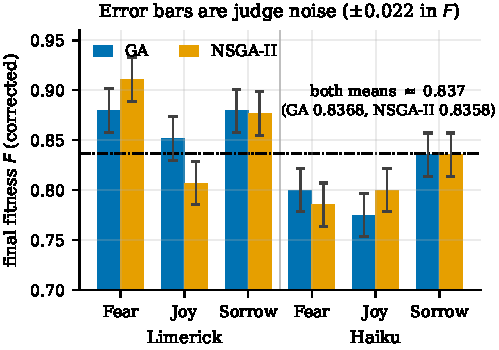
\includegraphics[width=\columnwidth]{fig_ga_vs_nsga.pdf}
\caption{Final fitness by condition. The two algorithms are separated by
$0.0010$ on average. Error bars show the judge noise measured in
Section~\ref{sec:judge} ($\pm 0.0218$ in $F$); the full span of one bar
($0.044$) exceeds every between-algorithm gap except the largest ($0.0446$).}
\label{fig:ga}
\end{figure}

Table~\ref{tab:results} and Fig.~\ref{fig:ga} give the comparison. Mean final
fitness is $0.8368$ (GA) against $0.8358$ (NSGA-II), a difference of $0.0010$.
On the uncorrected figures the difference is $0.0021$ in the same direction. The
GA wins three cells, NSGA-II two, and one is an exact tie. An exact two-sided
Wilcoxon signed-rank test drops the tied pair and is run on the remaining five,
giving $p = 1.0$. This test has very little power here: with five pairs the
smallest attainable two-sided $p$ is $0.0625$, so even five unanimous pairs could
not have reached $p<0.05$. The accurate reading is therefore not ``the test found
no difference'' but ``six pairs cannot show one''; the sign pattern (three,
two, one tie) is simply what no effect looks like.

Separating the fitness terms is more informative than the scalar. On judge
quality $\Qb$, NSGA-II is marginally ahead ($0.875$ versus $0.867$, two wins to
one with three ties); on structure $S$ the GA is ahead ($0.858$ versus $0.833$),
as the constraint-handling design predicts. Both differences are small --- the
$\Qb$ gap is a sixth of one judge step ($0.05$) --- and we do not test them,
since three of six $\Qb$ pairs are tied. The pattern is at least consistent with
each algorithm doing slightly better on the terms it actually selects on, and
with the scalar $F$ averaging two small opposing effects into almost nothing.

Resource use does not separate the two either. Wall-clock time is dominated by
rate-limit waiting (roughly $50$--$57$\,s per wait), so it is not a meaningful
comparison; token counts per run are similar across arms.

The honest summary is that with this instrument, at this sample size, there is no
evidence that the choice between these two algorithms matters. The next section
asks whether this instrument could have shown a difference at all.

% =====================================================================
\section{Is the Judge the Bottleneck?}\label{sec:judge}
% =====================================================================
A null result is uninformative if the fitness function cannot discriminate. We
therefore validated the judge directly. Three groups of poems were scored by the
same judge model with one shared four-dimension rubric (imagery, literary
devices, originality, coherence), so that all groups sit on one scale:
\textbf{(A)} 30 published human poems, 15 haiku by Bash\=o, Buson, Issa, Shiki,
S\=oseki and Chiyo, and 15 canonical English limericks, mostly by Edward Lear;
\textbf{(B)} 10 controls written to be bad in specific ways (bland, incoherent,
maximally clich\'ed, emotionally flat) while keeping correct form; and
\textbf{(C)} the 13 evolved poems. Each of the 53 poems was scored three times,
giving 159 judge calls. Group~(A) is reported only in aggregate.

\subsection{The judge discriminates}
\begin{figure}[t]
\centering
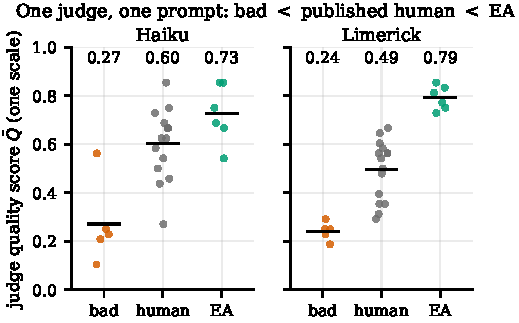
\includegraphics[width=\columnwidth]{fig_judge_groups.pdf}
\caption{Per-poem mean judge score by group on one scale. The ordering is
bad $<$ published human $<$ evolved for both forms. Points are poems; bars are
group means.}
\label{fig:groups}
\end{figure}

Fig.~\ref{fig:groups} shows the result. The judge orders the groups correctly and
separates published human poems from deliberately bad ones for both forms
(Mann-Whitney $U$ \cite{mann1947}, two-sided, on per-poem means: haiku $0.604$
versus $0.271$, $p = 0.005$; limerick $0.494$ versus $0.242$, $p = 0.001$). The
fitness function is not noise. Whatever explains the null result in
Section~\ref{sec:results}, it is not a judge that cannot tell poems apart.

\subsection{But it has a style preference}
The evolved poems outscore the published human ones in both forms. For haiku the
gap is not significant ($0.726$ versus $0.604$, $p = 0.078$). For limericks it is
large and unambiguous: $0.792$ versus $0.494$, $p = 0.0005$, with every one of
the six evolved limericks scoring above every one of the fifteen canonical ones.

That ordering should not be taken at face value, and the dimension breakdown
(Table~\ref{tab:dims}) shows why. Coherence is identical between the two groups
($4.72$ versus $4.73$). The entire gap comes from imagery ($+1.36$), literary
devices ($+1.82$) and originality ($+1.59$). A Lear limerick is deliberately
plain: its effect depends on timing and absurdity, not on metaphor density. The
rubric has no dimension for humour, wit or comic timing, so it scores the one
thing the form is built around at zero weight, and rewards ornamentation instead.
This is a concrete, measurable instance of the judge-bias concern raised in the
LLM-as-a-judge literature \cite{zheng2023,wang2024fair}, and it is a property of
the \emph{rubric}, which makes it fixable.

\begin{table}[t]
\caption{Sub-score means (1--5) for limericks, evolved versus published human.
The gap is entirely in ornamentation, not in coherence.}
\label{tab:dims}
\centering\footnotesize
\begin{tabular}{lccc}
\toprule
Dimension & Evolved & Human & Difference \\
\midrule
Imagery           & 4.33 & 2.98 & $+1.36$ \\
Literary devices  & 4.11 & 2.29 & $+1.82$ \\
Originality       & 3.50 & 1.91 & $+1.59$ \\
Coherence         & 4.72 & 4.73 & $-0.01$ \\
\bottomrule
\end{tabular}
\end{table}

\subsection{And it is unstable}
\begin{figure}[t]
\centering
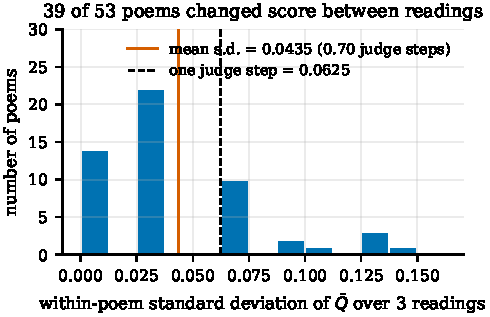
\includegraphics[width=\columnwidth]{fig_judge_noise.pdf}
\caption{Spread of the three readings of each poem. Most poems do not receive
the same score twice, and the mean spread is close to one full judge step.}
\label{fig:noise}
\end{figure}

The same poem, the same prompt and the same model do not give the same score.
Of the 53 poems, 39 ($73.6\%$) changed score between identical readings
(Fig.~\ref{fig:noise}). The mean within-poem standard deviation is $0.0435$,
which is $0.70$ of one judge step; the worst poem has a standard deviation of
$0.144$ and a range of $0.25$.

This is the finding that reframes the paper. A single judge reading carries
weight $0.5$ in~\eqref{eq:fitness}, so a standard deviation of $0.0435$ in $\Qb$
is $\pm 0.0218$ in $F$. The difference we set out to measure is $0.0010$. The
measurement error is roughly twenty times the effect, and the standard deviation
of a GA-minus-NSGA-II difference from judge noise alone is $0.031$ --- larger than
four of the six observed per-cell gaps, and about equal to a fifth. Under this noise model, detecting an
effect of the observed size at $80\%$ power would require on the order of $7{,}000$
matched pairs. No reasonable experiment will do that, which means the right
response is not more runs but a better instrument.

Averaging $k$ independent readings reduces the noise by $\sqrt{k}$: three
readings bring the contribution to $F$ down to $\pm 0.0126$. That is the single
change with the largest effect on what this pipeline can measure, and it costs
only judge calls.

\subsection{A case where the fitness function was wrong}
One poem was rejected by the user, in the GA haiku/joy cell, and re-run. The
production fitness scored the rejected poem \emph{higher} than its accepted
replacement ($F = 0.7917$ versus $0.7750$). The calibration judge, scoring blind
on the shared rubric, ranks them the other way ($0.583$ versus $0.667$). On the
only case in this study where an independent human verdict exists, the human and
the calibration rubric agree with each other and disagree with the fitness
function being optimised. One case proves nothing, but it points in the same
direction as the rest of this section.

% =====================================================================
\section{Threats to Validity}\label{sec:threats}
% =====================================================================
\textbf{One run per cell.} Each cell is a single run, so per-cell differences
cannot be separated from run-to-run variation. We report the resulting null as a
null, not as equivalence. Section~\ref{sec:judge} quantifies the cost: at the
observed effect size, no feasible number of replicates would settle the question
without first reducing judge noise.

\textbf{Noise is measured with a different rubric.} The noise figures come from
the four-dimension calibration rubric (step $0.0625$), not from the
five-dimension production rubric (step $0.05$). We assume the two are comparably
noisy, which is an assumption and not a measurement; the Phase~II logs record
every individual reading so it can be checked directly.

\textbf{A single judge family.} One judge model, one provider. Position and
self-enhancement biases \cite{zheng2023,wang2024fair} are not controlled, and
both the generator and the judge are open-weight models that may share training
data. Cross-model judging is left to future work.

\textbf{The rubric omits humour.} As shown above, the limerick result is a
property of the rubric rather than of the poems. The comparison with human
limericks should be read as evidence about the judge, not as evidence that
evolved limericks are better than Lear's.

\textbf{The apostrophe defect perturbed the search.} The within-run effect cannot
be reversed offline, and in one run it touched the majority of evaluated
candidates.

\textbf{One human verdict per run.} The only human signal collected is a single
accept/reject decision, made by the first author, who was not blind to the
condition. A blind expert rating of the final poems is the obvious next
measurement and has not yet been done.

\textbf{Two models, one language.} Results may not transfer to other model
families, other poetic traditions or other languages.

% =====================================================================
\section{Committed Protocol for the Next Phase}\label{sec:phase2}
% =====================================================================
The diagnosis above prescribes the fix, and the fix is implemented and committed
rather than proposed. The repository contains, behind a single flag that leaves
the original behaviour reachable: (i) the judge averaged over three independent
readings per poem, with unreadable replies skipped rather than silently replaced
by a middle score; (ii) apostrophe normalisation applied to the text before
scoring only, leaving the stored poem untouched; (iii) three replicates per cell
(36 runs), with completed runs skipped on restart so a rate-limited session can
resume; and (iv) per-candidate logging, so that selection pressure, not merely
final fitness, can be inspected. Phase~I logs are written to a separate directory
and are never modified. A test run on the live API confirms the averaging path
end to end; the full grid has not yet been run, and no Phase~II result is claimed
in this paper.

Two further changes are deliberately \emph{not} bundled with the measurement fix,
because changing the measuring instrument and the algorithms in the same step
would make the comparison uninterpretable: adding humour and wit to the judge
rubric, and correcting two NSGA-II implementation quirks (tie-breaking by list
order, and a best-so-far tracker that can report a poem other than the one
presented).

% =====================================================================
\section{Conclusion}
% =====================================================================
Given the same language model, the same judge and the same budget, we find no
evidence that NSGA-II produces better poems than a simple elitist GA: a gap of
$0.0010$ in mean fitness across twelve conditions, with wins split evenly. The
more useful result is why that question could not be answered as posed. The LLM
judge serving as the fitness function is valid in the coarse sense --- it ranks
deliberately bad poems below published human ones --- but it is unstable, with
$73.6\%$ of poems changing score between identical readings and a noise
contribution to fitness some twenty times the effect under study, and it carries
a measurable preference for ornate writing that penalises forms whose craft lies
in plainness.

For practitioners building LLM-in-the-loop evolutionary systems, the implication
is concrete: report the noise of your judge before reporting the benefit of your
algorithm. A comparison between search algorithms is only meaningful above the
noise floor of the fitness function, and in this pipeline that floor sat an order
of magnitude above the effect everyone would have been tempted to report.

\section*{Reproducibility}
Code, logs, prompts, the full per-run workbook and the judge-validation data are
available at \url{https://github.com/sakthicr/LLMMM}.

\bibliographystyle{unsrt}
\bibliography{refs}
\end{document}
